\PassOptionsToPackage{table}{xcolor}
\documentclass[12pt, a4paper]{article}
\usepackage{tkz-base}
\usepackage{tkz-euclide}
\usepackage{tikz}
\usepackage{xcolor}
\usepackage{multirow} 
\usepackage{flafter} 
\usetikzlibrary{arrows.meta}
\usepackage[left=2cm, right=2cm, top=2cm, bottom=2cm]{geometry}
\usepackage[brazil]{babel}
\usepackage[utf8]{inputenc}
\usepackage{color}
\usepackage{indentfirst}
\usetikzlibrary{angles, quotes}
\usepackage{amssymb}
\usepackage{amsmath}
\usepackage{pst-eucl}
\usepackage{tabularx,ragged2e,booktabs}
\usepackage{ragged2e,microtype}
\usepackage{array} % for '\newcolumntype' macro
% Define two new column types:
% (a) for full-width columns:
\newcolumntype{L}{@{} >{\RaggedRight}p{\dimexpr12cm+2\tabcolsep+1\arrayrulewidth\relax} @{}}
% (b) for half-width columns:
\newlength\mylen
\settowidth\mylen{$4.$\space} % amount of hanging indentation
\newcolumntype{P}[1]{>{\RaggedRight\hangafter1\hangindent\mylen}p{#1}}
\usepackage{float}
\usepackage{hyperref}
\usepackage[paper=portrait,pagesize]{typearea}
\usepackage{calrsfs}
\usepackage{mathtools}
\newcommand\myeq{\stackrel{\mathclap{\tiny\mbox{Bayes}}}{=}}
\usepackage{hyperref}
\usepackage{xurl}
\newcommand{\stackwords}[2]{\begin{tabular}[t]{@{}l@{}}#1\\#2\end{tabular}}
\usepackage{graphicx} 
\usepackage{subcaption} %  for subfigures environments 
\usepackage{pifont}
\begin{document}
	
	\begin{titlepage}
		\begin{center}
			{\large \textbf{Universidade Federal do Rio de Janeiro}}
			
			\vspace{0.2cm}
			
			{\large \textbf{Curso de Ciência da Computação}}
			
			\vspace{6.08cm}%%%%%%%%%%%%%%%%%%%%%%%%%%%%%%%%
			
			
			{\large \textbf{Catálogo de Estrelas até 23 parsecs do Sol}}\\
			{\normalsize \textbf{Trabalho de Iniciação Científica}}
			
			\vspace{6.08cm}%%%%%%%%%%%%%%%%%%%%%%%%%%%%%%%%
			\begin{tabbing}
				\hspace{7cm}\textbf{Alunas: \stackwords{Helena Serrano Cardoso da Costa}{Laura Serrano Cardoso da Costa}}
			\end{tabbing}
			
			\vspace{6.08cm}%%%%%%%%%%%%%%%%%%%%%%%%%%%%%%%%
			
			\textbf{2024}
		\end{center}	
	\end{titlepage}
	
	\newpage
	\listoffigures
	\listoftables
	\tableofcontents
	
	\newpage
	
	\section{Introdução}
	
	Nosso trabalho tem como objetivo construir um banco de dados com informações, majoritariamente provenientes do Catálogo Gaia, de estrelas próximas do Sol. Foram consideradas estrelas distantes no máximo $23$ parsecs do Sol ($23$ parsecs equivalem a $75.016$ anos-luz ou $7.097\cdot 10^{14}$ quilômetros). Além disso, também foram utilizadas informações do catálogo Hipparcos.
	
	Hipparcos é um satélite que foi lançado pela Agência Espacial Europeia (ESA) em 18 de agosto de 1989. A missão se deu como concluída em 1993.
	
	O gigantesco survey Gaia, utilizado neste trabalho, é um dos mais impactantes na Astronomia nos últimos anos. O telescópio Gaia foi lançado, também pela ESA, em 19 de dezembro de 2013. O primeiro catálogo proveniente da Missão Gaia com mais de um bilhão de estrelas foi publicado em 14 de setembro de 2016. Esta foi a maior pesquisa de objetos celestes até a data.

	\begin{figure}[H]
		\begin{subfigure}{.5\textwidth}
			\centering
			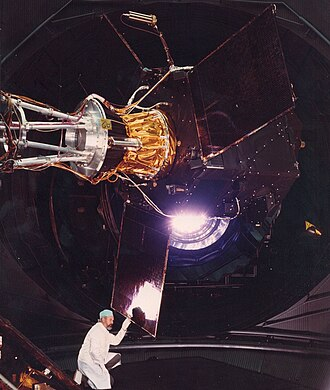
\includegraphics[width=.7\linewidth]{Hipparcos.png}
			\caption*{Hipparcos}
		\end{subfigure}%
		\begin{subfigure}{.5\textwidth}
			\centering
			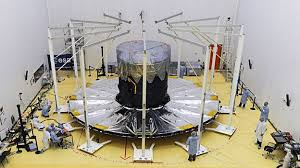
\includegraphics[width=1\linewidth]{Gaia.png}
			\caption*{Gaia}
		\end{subfigure}
		\caption{Telescópios Espaciais}
	\end{figure}

	No banco de dados criado neste trabalho, foram incluídos todos os registros que puderam ser obtidos do \href{https://gea.esac.esa.int/archive/}{Gaia Archive}, somente limitado pela capacidade de seleção da ferramenta (de 2000 registros). Trabalhamos com três arquivos de dados: um proveniente do catálogo Gaia, do tipo csv, com 1774 estrelas; um proveniente do catálogo Hipparcos, do tipo dat, com 118218 estrelas; e outro proveniente do \href{http://www.exoplanet.eu/}{The Extrasolar Planet Encyclopedia}, do tipo csv, contendo 5553 exoplanetas (planetas fora do Sistema Solar).
	
	A partir das informações contidas nestes arquivos, foi possível calcular algumas propriedades de cada estrela, como magnitude e índice de cor, e plotar essas propriedades em diagramas HR, que também foram armazenados no banco de dados.
	Também relacionamos os dados do Gaia com os do catálogo de exoplanetas. Ou seja, para cada estrela, proveniente do Gaia, obtivemos as informações, como massa e semieixo maior, dos planetas que orbitam ao seu redor. 
	
	Os dados do Gaia superam, em precisão, os dados do catálogo Hipparcos, e somente algumas das 1774 estrelas contidas no Gaia também estão no Hipparcos. Dessa forma, nosso trabalho se propõe a fazer um cruzamento de dados: algumas informações mais tradicionais, que são encontradas somente no Hipparcos, serão acrescentadas às estrelas Gaia que estejam, simultaneamente, nos dois catálogos. Logo, não é de interesse, neste trabalho, manter na base de dados as estrelas que estão somente no catálogo Hipparcos, mas acrescentar às estrelas provenientes do Gaia informações valiosas presentes apenas no Hipparcos.
	
	O interesse na obtenção destas propriedades e diagramas HR de estrelas próximas do Sol é astrobiológico: dentre as estrelas selecionadas, aquelas que tiverem potencial de ter uma zona habitável (isto é, uma região em que um planeta orbitando ao seu redor possa abrigar vida) serão estudadas em mais detalhes em uma pesquisa que utilizará esta base de dados. 
	
	\section{Conceitos de Astronomia usados no Tratamento do Dataset
	}
	\subsection{Esfera celeste}
	É uma esfera imaginária em volta da Terra, sem raio definido, que representa a projeção das estrelas como são vistas do nosso planeta. Os astrônomos mais antigos acreditavam que as estrelas estavam a uma mesma distância da Terra, como se estivessem “incrustadas” nesta esfera.

	\begin{figure}[h]
		\centering
		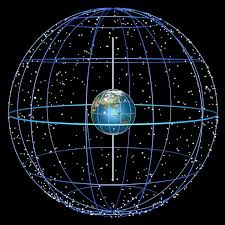
\includegraphics[width=0.37\textwidth]{celestial_sphere.png}
		\caption{Esfera Celeste}
		\label{fig:Esfera_Celeste}
	\end{figure}

	\subsection{Ponto Áries}
	
	O Ponto Áries, também chamado Ponto Vernal,	é um ponto do Equador celeste, ocupado pelo Sol quando passa do hemisfério
	sul celeste para o hemisfério norte celeste, definindo o equinócio de primavera do hemisfério norte (mais ou menos em 22 de março).

	\subsection{Ascensão reta $(\alpha)$}
	
	É o ângulo medido, sobre o equador celeste, do Ponto Vernal (ou Ponto Áries) ao meridiano do astro. É um conceito análogo ao de latitude geográfica.

	\begin{figure}[H]
		\centering
		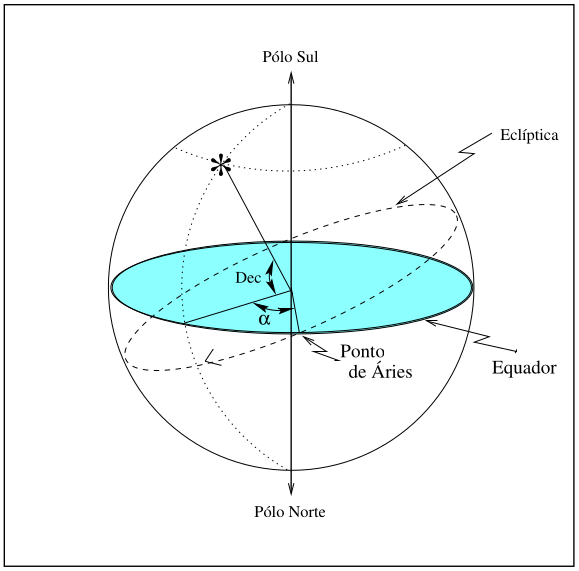
\includegraphics[width=0.5\textwidth]{right_ascension_and_declination.png}
		\caption{Ascensão Reta e Declinação}
	\end{figure}

	\subsection{Declinação $(\delta)$}
	É a medida do ângulo, sobre o meridiano do astro, que vai do equador celeste ao astro. É um conceito análogo ao de longitude geográfica (ver figura acima).
	
	\subsection{Semi-eixo maior}
	Semi-eixo maior da elipse descrita pela órbita do planeta ao redor da estrela. A estrela orbitada é um dos focos desta elipse.

	\begin{figure}[H]
		\centering
		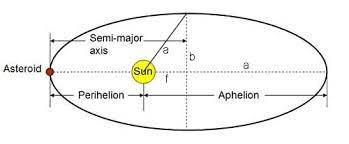
\includegraphics[width=0.7\textwidth]{semi_major_axis.png}
		\caption{Semi eixo maior}
	\end{figure}

	\section{Datasets}
	
	Os arquivos de dados com os quais o banco de dados foi populado foram obtidos do Gaia Archive, de um arquivo pessoal (\verb|HIP_MAIN.DAT|) e do The Extrasolar Planet Encyclopedia.
	
	Colunas contidas no csv extraído do Gaia Archive:
	
	ra (tipo numeric(65, 30)):
	Ascenção reta. É a primeira coordenada da localização da estrela.
	
	dec (tipo numeric(65, 30)):
	Declinação. É a segunda coordenada da localização da estrela.
	
	designation (tipo string): 
	Designação única para cada estrela no Gaia.
	
	ruwe (tipo numeric(65, 30))
	Basicamente é a medida da variação do brilho da estrela. Permite determinar se a estrela possui uma companheira binária.
	
	\verb|distance_gspphot| (tipo numeric(65, 30)):
	Distância medida em parsecs do Sol.
	
	parallax (tipo numeric(65, 30)):
	O deslocamento aparente de uma estrela por conta da mudança da posição da Terra em relação ao Sol.
	
	\verb|phot_g_mean_mag| (tipo numeric(65, 30)):
	Tipo de magnitude (brilho intrínseco) da banda g.
	
	\verb|phot_rp_mean_mag| (tipo numeric(65, 30)):
	Tipo de magnitude (brilho intrínseco) da banda rp.
	
	\verb|phot_bp_mean_mag| (tipo numeric(65, 30)):
	Tipo de magnitude (brilho intrínseco) da banda bp.
	
	Colunas contidas no csv \verb|HIPPARCOS_MAIN.DAT|
	
	HIP (tipo int):
	Identificação única da estrela no Hipparcos.
	
	Vmag (tipo numeric(65, 30)):
	Magnitude V (brilho intrínseco) 
	
	RAdeg (tipo numeric(65, 30)):
	Ascenção reta, que é a primeira coordenada da posição da Estrela.
	
	DEdeg (tipo numeric(65, 30)):
	Declinação, que é a segunda coordenada da posição da Estrela.
	
	Plx (tipo numeric(65, 30)):
	O deslocamento aparente de uma estrela por conta da mudança da posição da Terra em relação ao Sol.
	
	pmRA (tipo numeric(65, 30)):
	Medida do movimento físico próprio de cada estrela, em relação ao equador celeste.
	
	pmDE (tipo numeric(65, 30)):
	Medida do movimento físico próprio de cada estrela, em relação ao meridiano da Estrela.
	
	BTmag (tipo numeric(65, 30)):
	Magnitude B específica do Hipparcos, chamada de magnitude de Tycho Brahe.
	
	VTmag (tipo numeric(65, 30)):
	Magnitude V específica do Hipparcos, chamada de magnitude de Tycho Brahe.
	
	\verb|B_V| (tipo numeric(65, 30)):
	Índice de cor (medida de temperatura da estrela) específica do Hipparcos.
	
	Colunas contidas no arquivo extraído do The Extrasolar Planet Encyclopedia:
	
	name (tipo string):
	Nome do planeta.
	
	mass (tipo numeric(65, 30)):
	Massa do planeta.
	
	\verb|semi_major_axis| (tipo numeric(65, 30)):
	Semi-eixo maior da elipse descrita pela órbita do planeta ao redor da Estrela.
	
	\verb|orbital_period| (tipo numeric(65, 30)): 
	Tempo que o planeta leva para dar uma volta completa em torno da Estrela.
	
	\section{Tratamento dos Datasets}
	
	\subsection{Gaia e Hipparcos}
	
	Primeiramente, fizemos o download dos arquivos nos endereços especificados anteriormente. Após isso, criamos um banco de dados auxiliar e, dentro deste banco, criamos duas tabelas, Gaia e Hipparcos. Cada arquivo baixado foi carregado em uma destas tabelas. Foi usada uma consulta SQL left outer join para poder adicionar às estrelas Gaia, presentes nos dois catálogos, informações extras que estão presentes apenas no Hipparcos. O resultado desta consulta foi gravado em um arquivo no formato csv e utilizado para popular a tabela Star do banco de dados \verb|Catalogo_Gaia|. Porém, em vez de a consulta retornar algumas centenas de Estrelas, como era esperado, retornou apenas algumas dezenas delas. Assim, decidimos carregar os dados do Hipparcos e do Gaia diretamente no BD, sem tratamento, nas tabelas \verb|Source_Gaia| e \verb|Source_Hipparcos|, respectivamente. Fizemos essa escolha porque precisávamos de um número grande de registros de estrelas para que os diagramas HR pudessem fazer sentido. A tentativa de relacionar os registros dos dois catálogos foi feita através de uma consulta, sem que o esquema do banco de dados fosse alterado.
	Uma possível solução para conseguir relacionar corretamente os dois catálogos seria a implementação de uma fórmula mais precisa para a conversão da ascensão reta e declinação das Estrelas. A fórmula que implementamos é uma simplificação de uma fórmula mais complexa e completa. Esta fórmula mais simples deveria funcionar para intervalos de tempos curtos (dezesseis anos). A suspeita que temos é de que a precisão dos dados do Gaia e Hipparcos é alta, o que não permite utilizar a fórmula simplificada para a transformação das coordenadas da época 2000.0 para a época 2016.0. Este trabalho continuará em andamento no próximo ano, e pretendemos fazer a correlação entre os registros dos dois catálogos de forma precisa.
	
	\subsection{Planetas Extrasolares}
	
	Baixamos um arquivo csv do The Extrasolar Planet Encyclopedia e carregamos estes dados em uma tabela auxiliar. Depois, fizemos uma left outer join com a tabela Hipparcos, para adicionar características das estrelas aos registros de planetas. Após isto, tentamos fazer outra left outer join, desta vez entre o resultado da consulta anterior e a tabela Gaia. O resultado destas duas consultas (feita na verdade através de uma única consulta com subconsulta aninhada) foi o de relacionar os registros dos planetas aos registros das estrelas no Gaia. Mas, novamente devido ao problema de transformação de coordenadas, não conseguimos obter o resultado esperado com essa consulta. Então, o resultado apenas da primeira consulta foi gravado em um arquivo no formato csv e utilizado para popular a tabela Planet (que se relaciona com a tabela \verb|Source_Hipparcos|) do banco de dados \verb|Catalogo_Gaia|.
	
	\section{Projeto do Banco de Dados}
	
	\subsection{Modelo Conceitual}
	\subsection{Modelo Lógico}
	\subsection{Modelo Físico}
	
	\section{Aplicação}
	
	O link a seguir direciona para o repositório do código do projeto no GitHub:
	
	\href{https://github.com/Laura-Costa/Catalogo_GAIA}{Catálogo GAIA} 
	\section{Considerações Finais}
	
	\newpage
	\section*{Referências}
	
	\vspace{20pt}
	
	[1] \url{https://tex.stackexchange.com/questions/282869/putting-two-figures-side-by-side}
	
	[2]
	\url{https://pt.wikipedia.org/wiki/Hipparcos}

	[3]
	\url{https://pt.wikipedia.org/wiki/Gaia_(sonda_espacial)}
	
	[4]
	\url{https://orionbearastronomy.com/2019/02/05/using-the-celestial-coordinates/}
	
	[5]
	\url{http://astro.if.ufrgs.br/}
	
	[6]
	\url{https://astronomy.stackexchange.com/questions/23773/can-one-approximate-the-semi-major-axis-of-an-orbit-as-the-average-orbital-dista}
	
\end{document}